%http://www.informatik.uni-freiburg.de/~frank/ENG/latex-course/latex-course-3/latex-course-3_en.html
\documentclass{beamer}

\usepackage{graphicx}
\usepackage{textpos}
\usepackage{amsmath}
\usepackage{bm}
\usepackage{color} % For my tc command
\usepackage[labelformat=empty]{caption}
%\usepackage{algorithmic} % Need to install texlive
\def\wl{\par \vspace{\baselineskip}}
\def\imp{\Rightarrow}
\newcommand\tc[1]{\textcolor{red}{\textbf{#1}}}

% Sorah Used This:
\usepackage{xcolor}

% See this for more themes and colors: http://www.hartwork.org/beamer-theme-matrix/
\usepackage{beamerthemeHannover} % Determines the Theme
\usecolortheme{seahorse}         % Determines the Color

\title{Tornado - Random Forests}
%\logo{
\includegraphics[width=1cm,height=1cm,keepspectration]{logo.png}}
\author[Arthur Lui\\Sorah Kang]{Arthur Lui \\ Sorah Kang}
\institute[Brigham Young University]{
  Department of Statistics\\
  Brigham Young University
}

%Setting %%%%%%%%%%%%%%%%%%%%%%%%%%%%%%%%%%%%%%%%%%%%%%%%%%%%%%%%%%%%%%%%%%%%%%%%%

%- 5pts Problem Statement and Understanding 
%    Does the report summary sufficiently describe the background of the problem?
%    Are the goals of the analysis clearly stated?
%
%- 15pts Describe the method/model(s) that are used.
%    Was a brief description of method/model used given in the report?
%    Were any greek letters used clearly defined?  
%    Were any explicit or implicit assumptions needed to use the model adequately 
%    explained? (Collinearity, Linearity, Independence)
%
%- 10pts Model Justification
%    Does the report give reasons for why the particular model was chosen?
%    Does the report describe why this model is appropriate for this data and how 
%    it solves the current problem?
%    Are the assumptions of the model justified (e.g. via exploratory analysis)?
%
%- 15pts Results
%    Does the report adequately answer the questions posed in the case study?
%    Were estimates of the parameters and their uncertainties given?
%    Were the parameters interpreted in the context of the problem?
%    Did the report summarize the main points of the results in non-statistical 
%    terms?
%
%- 5pts Conclusions
%
%    Did the report discuss other potential approaches to solving the problem?
%    Did the report discuss any shortcomings of the approach/model used?
%    Did the report provide suggestions for next steps in the analysis or further 
%    questions that may be of interest?

\begin{document}

  \frame{\titlepage}

  \section{Introduction} % Sorah
      \frame{
        \frametitle{Introduction}
        \begin{center}
        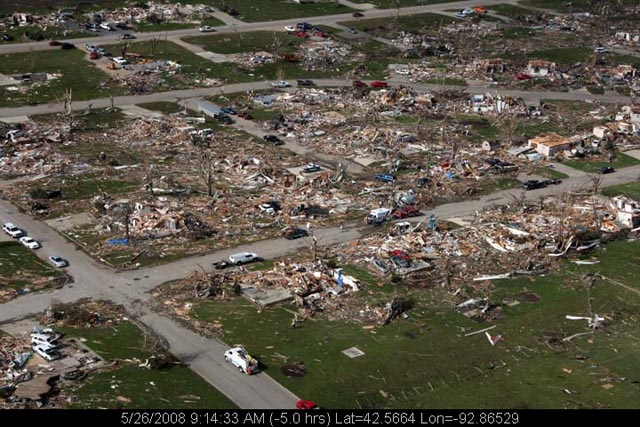
\includegraphics[height=7cm]{out/damage.jpg}
        \end{center}
      }
      
      \frame{
      \frametitle{Goal}
      The goal of this analysis is to develop an objective model for 
      classifying tornados
      }

  \section{Data} % Sorah
      \frame{
        \frametitle{Data}
        % where the data is from, what variables
        Data on tornados in 2012 from the Storm Prediction Center (SPC)
        \begin{itemize}
        \item Number - SPC Tornado Number
        \item Month - Numeric Month Value
        \item Day - Day of the Month
        \item Time - Time Tornado First Reported
        \item Fscale - Fujita Scale
        \item Loss - Rounded Total Dollar Property Loss (in millions)
        \item CropLoss - Rounded Total Dollar Crop Loss (in millions)
        \item Length - Length of impact (in miles)
        \item Width - Width of impact (in yards)
        \end{itemize}
      }
      \frame{
        \frametitle{Data}
          % some graphs of the data
          \begin{center}
          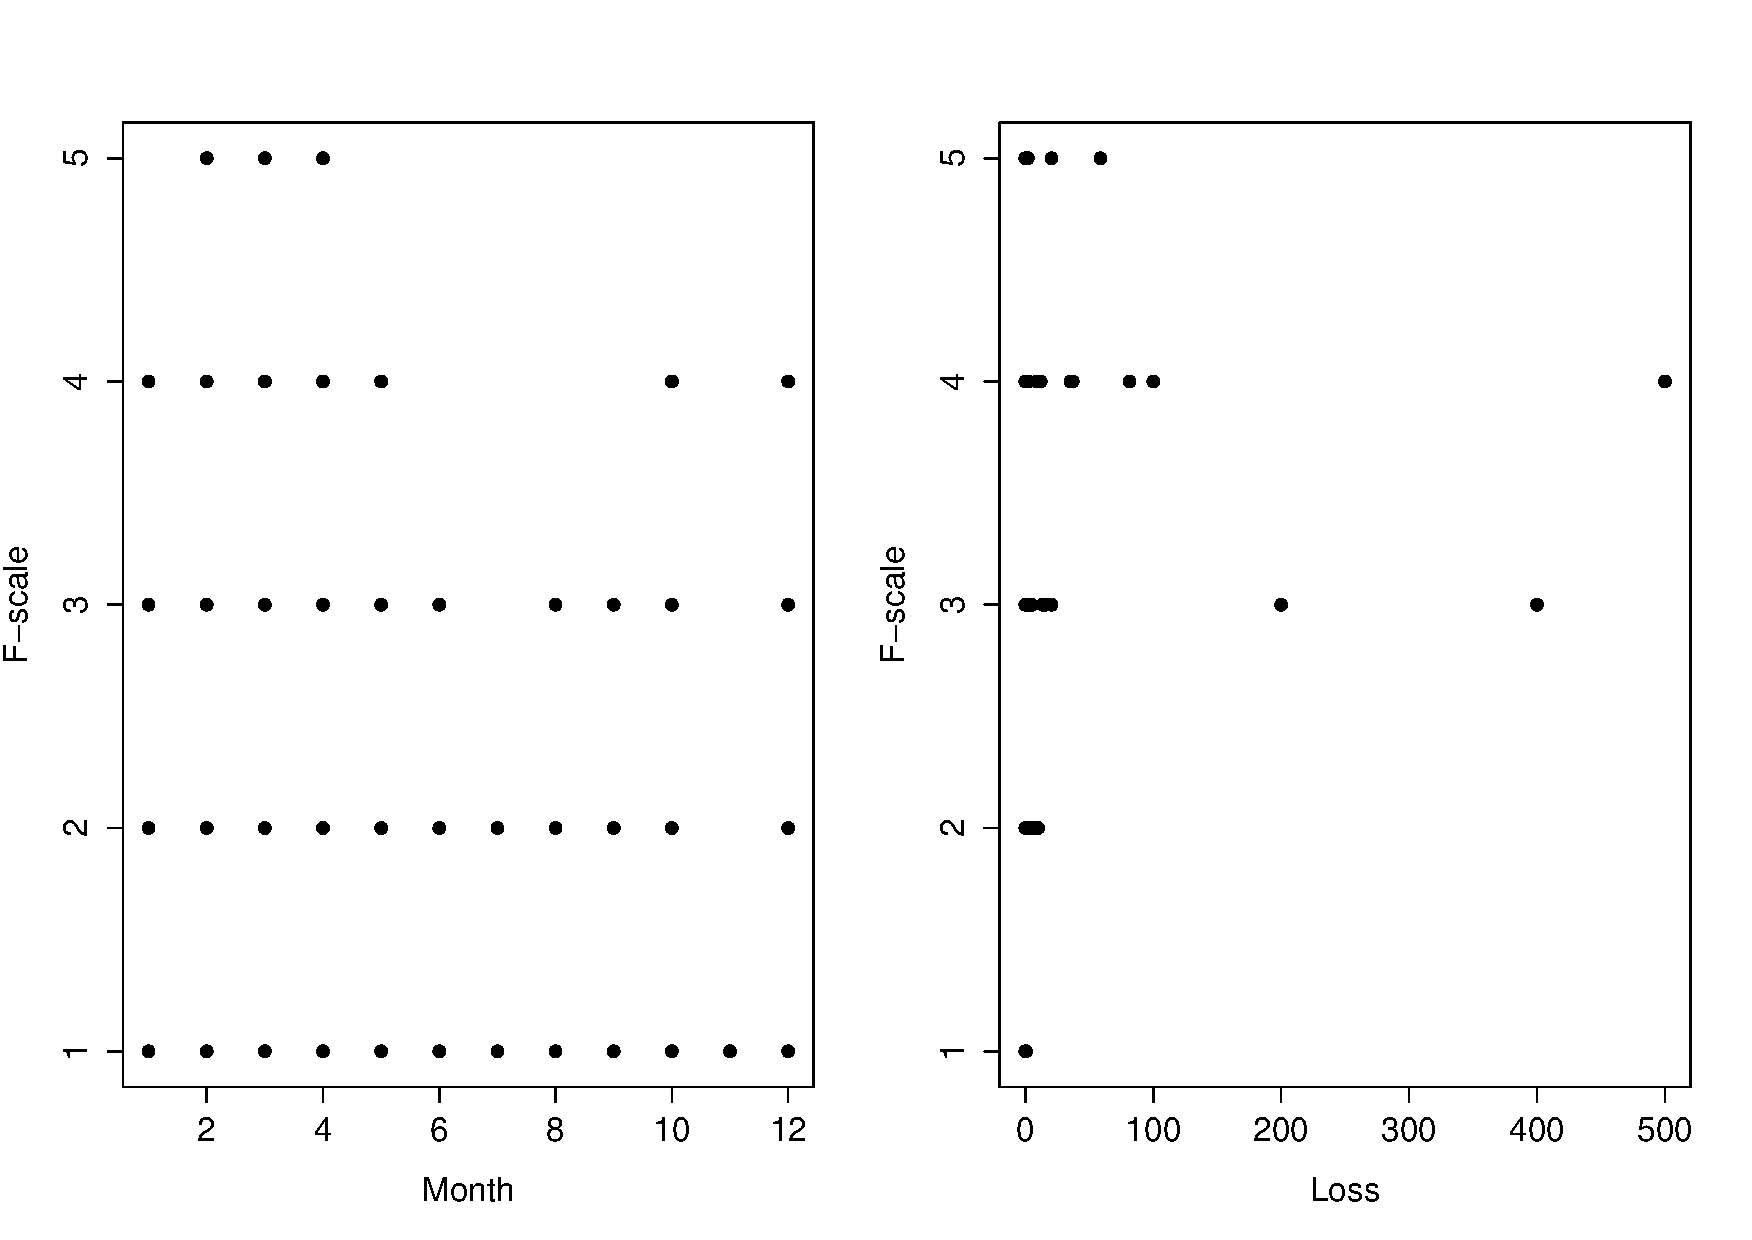
\includegraphics[height=6cm]{out/dat.pdf}
          \end{center}
          % table of how many obs per fscale
          \begin{table}[ht]
          \centering
          \begin{tabular}{l r r r r r r} \hline
          F-Scale & 0   & 1   & 2   & 3   & 4   & 5 \\ \hline
          Freq    & 578 & 242 & 100 & 32  & 5   & 0 \\  \hline
          \end{tabular}
          \end{table}
      }

      \frame{ % Sorah
        \frametitle{Data Cleaning}
        % give an example of repeated observations
        There were $23$ tornados that were repeated
        \pause
        \begin{table}[ht]
        \centering
        \begin{tabular}{r l l l l l l l} \hline
            &Number &Date    &State &F-scale &Injuries &Loss &Length\\ \hline
        120 &359692 &2/29/12 &IL    &2       &0        &0.05 &8.41\\
        {\color{red}121} &{\color{red}359692} &{\color{red}2/29/12} &{\color{red}IL}    
        &{\color{red}2}       &{\color{red}5}        &{\color{red}0.30} &{\color{red}25.12}\\
        122 &359692 &2/29/12 &KY    &2       &5        &0.25 &26.71\\ \hline
        \end{tabular}
        \end{table}
      }
   
    \section{Model: Random Forests} % Sorah
      \frame{
        \frametitle{Model}
        Random Forest - The idea is to create a multitude of trees (forest)
        \begin{enumerate}
        \item Take a bootstrap sample of size $n$.
        \item At each split, randomly sample $m<P$ variables
        \item Build a tree based on each set
          \begin{enumerate}
          \item At each node, identify variable that has most correlation with output
          \item Identify a cut point that leads to the greatest reduction in error
          \end{enumerate}
        \end{enumerate}
      }

      \frame{
        \frametitle{Random Forests}
        \begin{itemize}
        \item[+] Better predictive power than trees
          \begin{itemize}
          \item Choosing a subset of variables decorrelates the trees
          \end{itemize}
        \item[+] Gives us an objective way of classifying tornados
        \item[-] However, random forests are not very interpretable
        \end{itemize}
      }

      \frame{
        \frametitle{Model Assumptions}
          - For classification trees, we assume data is non-linear
          \begin{center}
          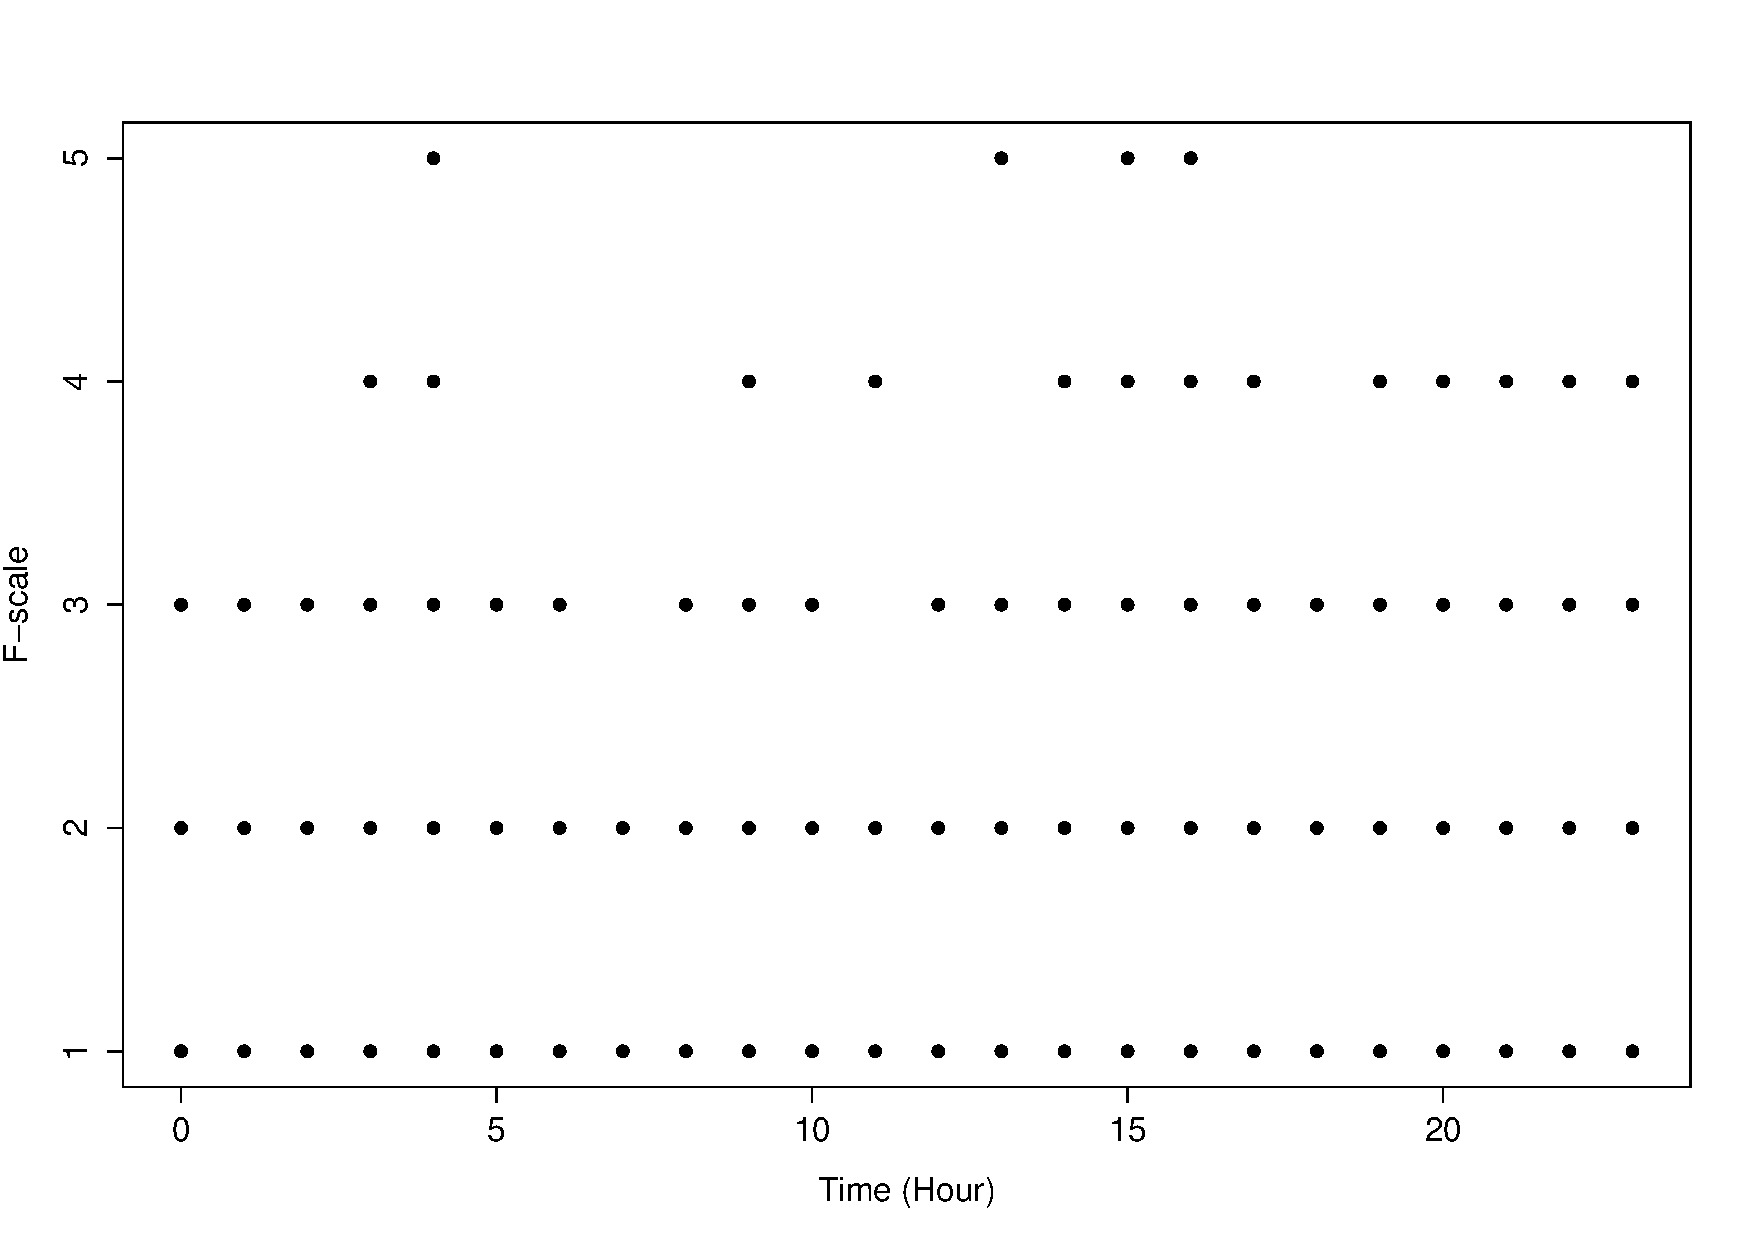
\includegraphics[height=7cm]{out/nonlinear.pdf}
          \end{center}
      }

%%%%%%%%%%%%%%%%%%%%%%%%%%%%%%%%%%%%%%%%%%%%%%%%%%%%%%%%%%%%%%%%%%%%%%%%%%%%%%%%%%%  
%       - Show your results? (But how?)
%       - How would a scientist use our model? (Using predictors and find Prediction)
%       - Plot while holding other variables constant, and changing Loss,
%         how the predicted Fscale changes.
%       - Include a picture of a forest  
%       - Include a tree. Using our model and a tree. 
%           (2 tress: Width and Loss, Width Length)
%       - Include Variable Importance    
%       - Show confusion matrix. Point out how Fscale classification error 
%         increases with Fscale.

  \section{Results}
     \frame{
      \frametitle{Most Important Variables}
      \center{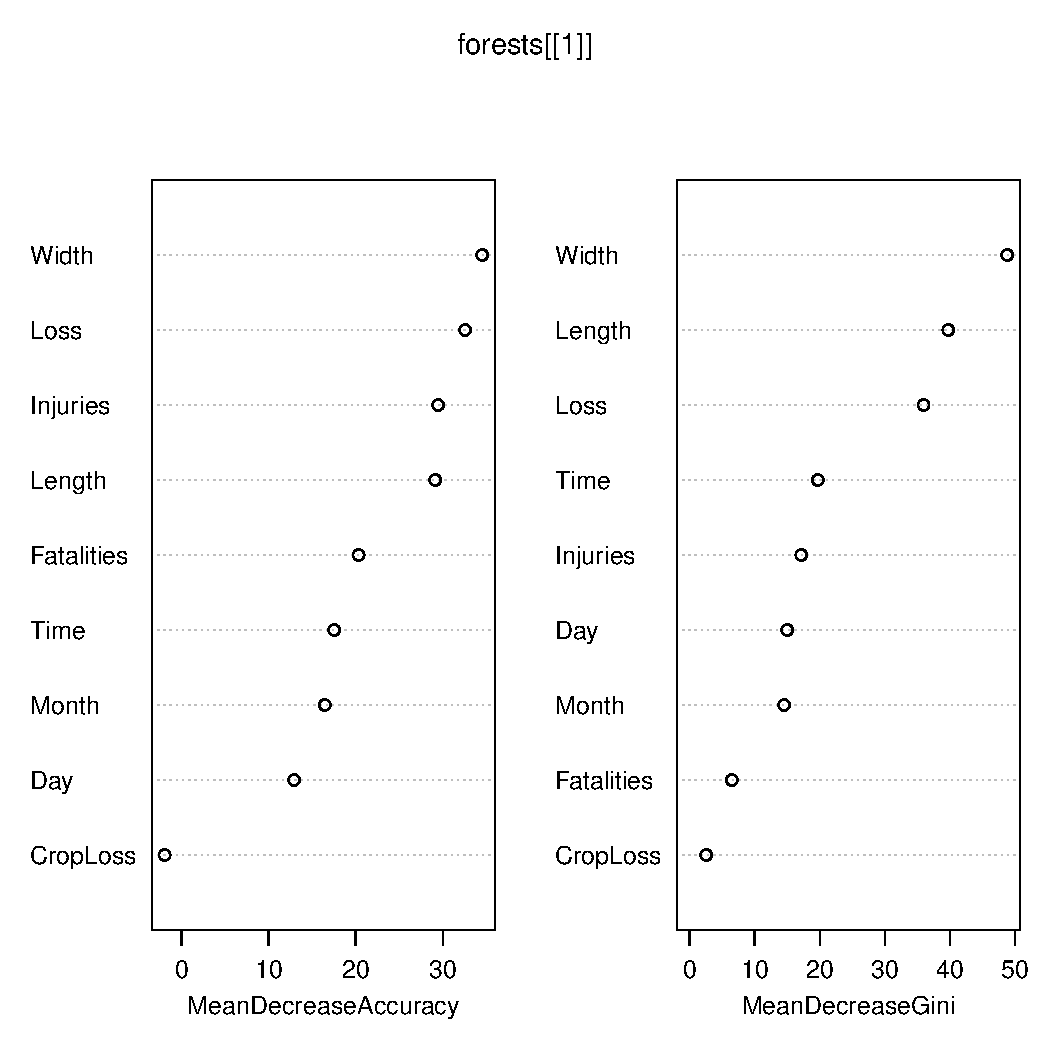
\includegraphics[scale=.35]{out/importance.pdf}}\\
      \small{The most important variables in predicting Fscale are: 
             Loss, Width, and Length.}
    }
   
    \frame{
      \frametitle{Tree}
      % I need some examples for each Fscale.
      \center{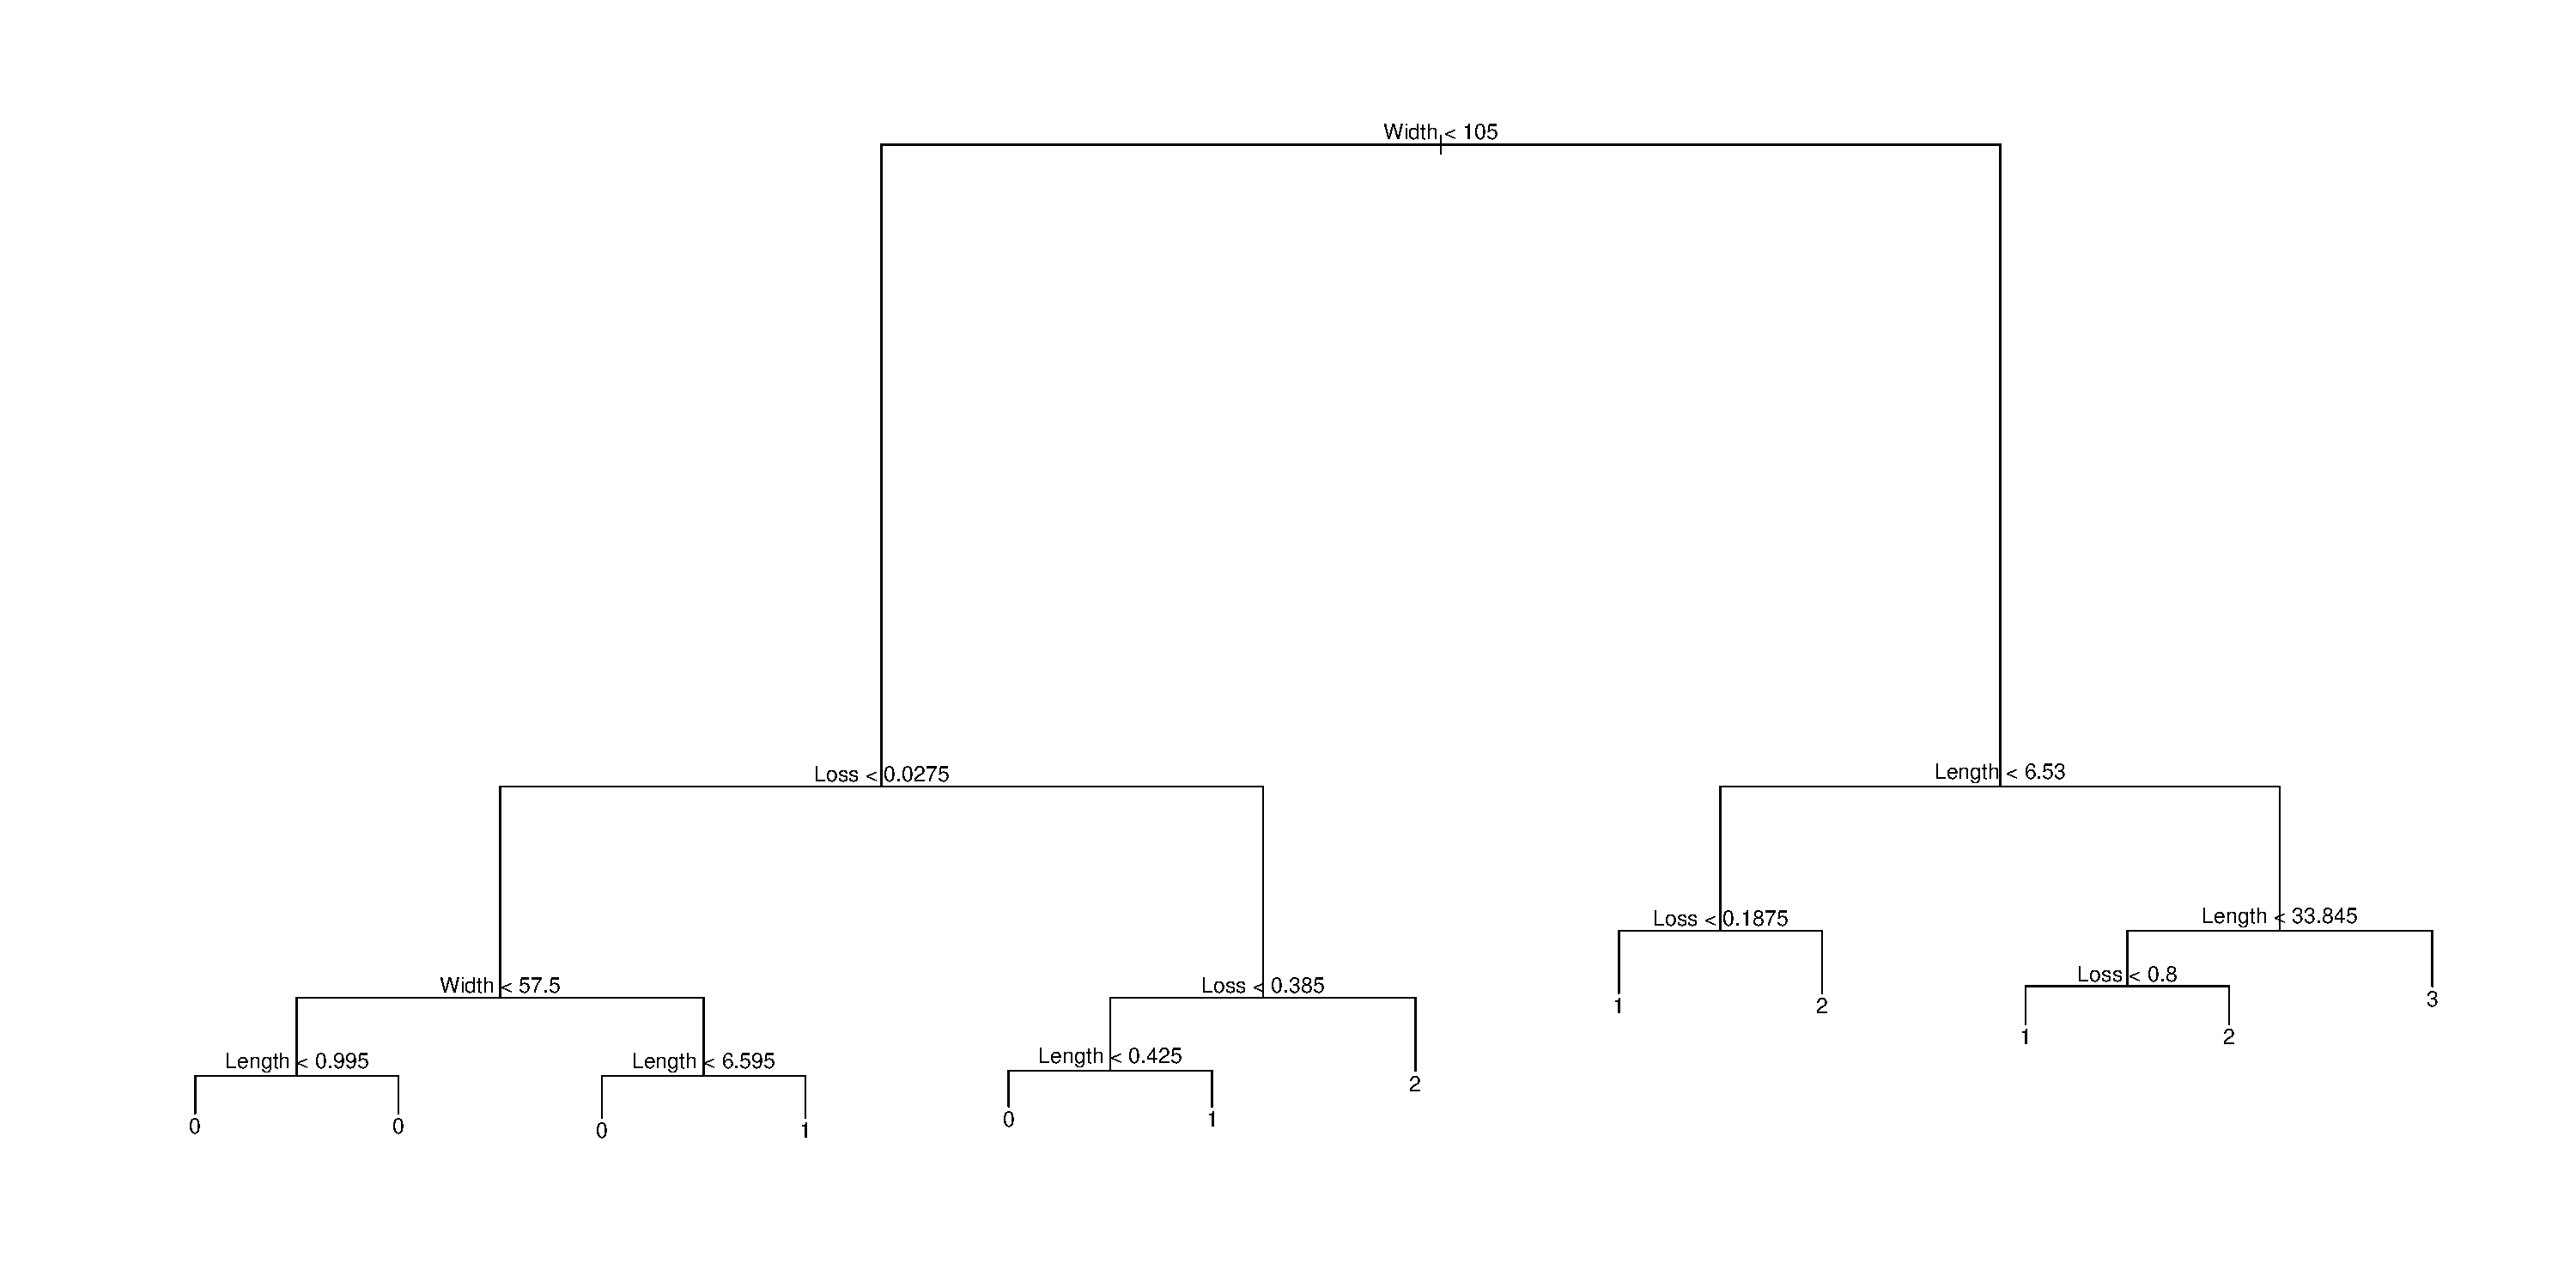
\includegraphics[scale=.2]{out/oneTree.pdf}}
      \small{How would a scientist use this model?}
    }

    \frame{
      \frametitle{Confusion Matrix}
      % latex table generated in R 3.0.3 by xtable 1.7-1 package
% Wed Apr  9 16:50:54 2014
\begin{table}[ht]
\centering
\begin{tabular}{rrrrrrr}
  \hline
 & 0 & 1 & 2 & 3 & 4 & class.error \\ 
  \hline
0 & 515.00 & 58.00 & 3.00 & 0.00 & 0.00 & 0.11 \\ 
  1 & 88.00 & 135.00 & 17.00 & 1.00 & 0.00 & 0.44 \\ 
  2 & 4.00 & 43.00 & 44.00 & 4.00 & 0.00 & 0.54 \\ 
  3 & 0.00 & 5.00 & 15.00 & 4.00 & 0.00 & 0.83 \\ 
  4 & 0.00 & 1.00 & 1.00 & 2.00 & 0.00 & 1.00 \\ 
   \hline
\end{tabular}
\end{table}

      \small{Note: Error rate is lower for small Fscales}
    }


  \section{Conclusions}
    \frame{
      \frametitle{Conclusions}
        \begin{itemize}
          \item Error Rate $\approx$ 26\%
          \item Objective and takes into account past data
          \item Predicts low Fscales well (because more data)
        \end{itemize}
    }

  \section{Future}
    \frame{
      \frametitle{Future}
        \begin{itemize}
          \item Need more data for Fscale = 4
          \item Compare different methods (e.g. trees, bagging, etc.)
        \end{itemize}  
    }

  \section{Teamwork}
    \frame{
      \frametitle{Teamwork}
        \begin{itemize}
          \item Did Analysis together
          \item Sorah:  Introduction, Model, Data
          \item Arthur: Results, Conclusions, Future
        \end{itemize}
    }
\end{document}
